% Options for packages loaded elsewhere
\PassOptionsToPackage{unicode}{hyperref}
\PassOptionsToPackage{hyphens}{url}
%
\documentclass[
  english,
  man,floatsintext]{apa6}
\usepackage{lmodern}
\usepackage{amssymb,amsmath}
\usepackage{ifxetex,ifluatex}
\ifnum 0\ifxetex 1\fi\ifluatex 1\fi=0 % if pdftex
  \usepackage[T1]{fontenc}
  \usepackage[utf8]{inputenc}
  \usepackage{textcomp} % provide euro and other symbols
\else % if luatex or xetex
  \usepackage{unicode-math}
  \defaultfontfeatures{Scale=MatchLowercase}
  \defaultfontfeatures[\rmfamily]{Ligatures=TeX,Scale=1}
\fi
% Use upquote if available, for straight quotes in verbatim environments
\IfFileExists{upquote.sty}{\usepackage{upquote}}{}
\IfFileExists{microtype.sty}{% use microtype if available
  \usepackage[]{microtype}
  \UseMicrotypeSet[protrusion]{basicmath} % disable protrusion for tt fonts
}{}
\makeatletter
\@ifundefined{KOMAClassName}{% if non-KOMA class
  \IfFileExists{parskip.sty}{%
    \usepackage{parskip}
  }{% else
    \setlength{\parindent}{0pt}
    \setlength{\parskip}{6pt plus 2pt minus 1pt}}
}{% if KOMA class
  \KOMAoptions{parskip=half}}
\makeatother
\usepackage{xcolor}
\IfFileExists{xurl.sty}{\usepackage{xurl}}{} % add URL line breaks if available
\IfFileExists{bookmark.sty}{\usepackage{bookmark}}{\usepackage{hyperref}}
\hypersetup{
  pdftitle={Graduate Statistics Semester Project},
  pdfauthor={Patrick Ihejirika1},
  pdflang={en-EN},
  hidelinks,
  pdfcreator={LaTeX via pandoc}}
\urlstyle{same} % disable monospaced font for URLs
\usepackage{graphicx,grffile}
\makeatletter
\def\maxwidth{\ifdim\Gin@nat@width>\linewidth\linewidth\else\Gin@nat@width\fi}
\def\maxheight{\ifdim\Gin@nat@height>\textheight\textheight\else\Gin@nat@height\fi}
\makeatother
% Scale images if necessary, so that they will not overflow the page
% margins by default, and it is still possible to overwrite the defaults
% using explicit options in \includegraphics[width, height, ...]{}
\setkeys{Gin}{width=\maxwidth,height=\maxheight,keepaspectratio}
% Set default figure placement to htbp
\makeatletter
\def\fps@figure{htbp}
\makeatother
\setlength{\emergencystretch}{3em} % prevent overfull lines
\providecommand{\tightlist}{%
  \setlength{\itemsep}{0pt}\setlength{\parskip}{0pt}}
\setcounter{secnumdepth}{-\maxdimen} % remove section numbering
% Make \paragraph and \subparagraph free-standing
\ifx\paragraph\undefined\else
  \let\oldparagraph\paragraph
  \renewcommand{\paragraph}[1]{\oldparagraph{#1}\mbox{}}
\fi
\ifx\subparagraph\undefined\else
  \let\oldsubparagraph\subparagraph
  \renewcommand{\subparagraph}[1]{\oldsubparagraph{#1}\mbox{}}
\fi
% Manuscript styling
\usepackage{upgreek}
\captionsetup{font=singlespacing,justification=justified}

% Table formatting
\usepackage{longtable}
\usepackage{lscape}
% \usepackage[counterclockwise]{rotating}   % Landscape page setup for large tables
\usepackage{multirow}		% Table styling
\usepackage{tabularx}		% Control Column width
\usepackage[flushleft]{threeparttable}	% Allows for three part tables with a specified notes section
\usepackage{threeparttablex}            % Lets threeparttable work with longtable

% Create new environments so endfloat can handle them
% \newenvironment{ltable}
%   {\begin{landscape}\begin{center}\begin{threeparttable}}
%   {\end{threeparttable}\end{center}\end{landscape}}
\newenvironment{lltable}{\begin{landscape}\begin{center}\begin{ThreePartTable}}{\end{ThreePartTable}\end{center}\end{landscape}}

% Enables adjusting longtable caption width to table width
% Solution found at http://golatex.de/longtable-mit-caption-so-breit-wie-die-tabelle-t15767.html
\makeatletter
\newcommand\LastLTentrywidth{1em}
\newlength\longtablewidth
\setlength{\longtablewidth}{1in}
\newcommand{\getlongtablewidth}{\begingroup \ifcsname LT@\roman{LT@tables}\endcsname \global\longtablewidth=0pt \renewcommand{\LT@entry}[2]{\global\advance\longtablewidth by ##2\relax\gdef\LastLTentrywidth{##2}}\@nameuse{LT@\roman{LT@tables}} \fi \endgroup}

% \setlength{\parindent}{0.5in}
% \setlength{\parskip}{0pt plus 0pt minus 0pt}

% Overwrite redefinition of paragraph and subparagraph by the default LaTeX template
% See https://github.com/crsh/papaja/issues/292
\makeatletter
\renewcommand{\paragraph}{\@startsection{paragraph}{4}{\parindent}%
  {0\baselineskip \@plus 0.2ex \@minus 0.2ex}%
  {-1em}%
  {\normalfont\normalsize\bfseries\itshape\typesectitle}}

\renewcommand{\subparagraph}[1]{\@startsection{subparagraph}{5}{1em}%
  {0\baselineskip \@plus 0.2ex \@minus 0.2ex}%
  {-\z@\relax}%
  {\normalfont\normalsize\itshape\hspace{\parindent}{#1}\textit{\addperi}}{\relax}}
\makeatother

% \usepackage{etoolbox}
\makeatletter
\patchcmd{\HyOrg@maketitle}
  {\section{\normalfont\normalsize\abstractname}}
  {\section*{\normalfont\normalsize\abstractname}}
  {}{\typeout{Failed to patch abstract.}}
\patchcmd{\HyOrg@maketitle}
  {\section{\protect\normalfont{\@title}}}
  {\section*{\protect\normalfont{\@title}}}
  {}{\typeout{Failed to patch title.}}
\makeatother
\usepackage{lineno}

\linenumbers
\usepackage{csquotes}
\ifxetex
  % Load polyglossia as late as possible: uses bidi with RTL langages (e.g. Hebrew, Arabic)
  \usepackage{polyglossia}
  \setmainlanguage[]{english}
\else
  \usepackage[shorthands=off,main=english]{babel}
\fi

\title{Graduate Statistics Semester Project}
\author{Patrick Ihejirika\textsuperscript{1}}
\date{}


\shorttitle{Semester Project}

\affiliation{\vspace{0.5cm}\textsuperscript{1} CUNY Brooklyn College}

\begin{document}
\maketitle

\hypertarget{background}{%
\section{Background}\label{background}}

Studies exploring the relationships between social interactions and the required underlying cognitive processes provide insight on mechanisms involved in the perception of others. This perception of others is influenced by outward egocentric projection, behavior interpretation \& stereotype formation. Hall and Schmid Mast (2007) and Kruger, Epley, Parker, and Ng (2005) found evidence that the intonation, cadence and amplitude of one's speech, enables vocal communication to be an effective medium of communicating one's thoughts over other methods of discourse.

The importance of vocal communication and its potential to portray the speaker's mental capacity serves as the foundation for the research conducted by (2015). Schroder \& Epley assessed whether and the extent that the perception of a person's mental capacity is influenced by the presence or absence of the person's voice over the course of 4 separate experiments. Seeing as how vocal communication is an effective method of communicating one's thoughts, Schroder \& Epley predicted that vocal speech will enable the portrayal of the speaker's mental capacity better than that of transcribed speech throughout the experiments.

\hypertarget{participants}{%
\subsection{Participants}\label{participants}}

Thirty nine professional recruiters from Fortune 500 companies were used. The average age of the recruiters was 30.85 years (SD = 6.24)

\hypertarget{material}{%
\subsection{Material}\label{material}}

We used R (Version 4.0.2; R Core Team, 2020) and the R-packages \emph{dplyr} (Version 1.0.7; Wickham et al., 2021a), \emph{ggplot2} (Version 3.3.5; Wickham, 2016), \emph{papaja} (Version 0.1.0.9997; Aust \& Barth, 2020), \emph{plyr} (Version 1.8.6; Wickham et al., 2021a; Wickham, 2011), \emph{pwr} (Version 1.3.0; Champely, 2020), \emph{readr} (Version 2.1.1; Wickham et al., 2021b), and \emph{tinylabels} (Version 0.2.1; Barth, 2021) for all our analyses.

\hypertarget{procedure}{%
\subsection{Procedure}\label{procedure}}

The thirty nine professional recruiters were presented with either orally recorded pitch presentations (audio pitch presentation condition) or the written pitch presentations (transcribed pitch presentation conditions) of eighteen University of Chicago MBA students. Upon completion of the pitch presentations, the recruiters were given a series of survey questions which asked for an evaluation of the candidate's intellect, impression left by the candidates and likelihood of hiring the candidates. Recruiter responses were placed along Likert scales which ordinally ranks responses between 0 to 10.

Questions evaluating the intellect of candidates asked the recruiters to rate \enquote{how competent the candidate seemed compared with an average candidate for an MBA-level position}, \enquote{how thoughtful the candidate seemed compared with an average candidate for an MBA-level position} \& \enquote{how intelligent the candidate seemed compared with an average candidate for an MBA-level position}. Responses to these questions were placed along Likert scales (0 = much less competent, 10 = much more competent), (0 = much less thoughtful, 10 = much more thoughtful), (0 = much less intelligent, 10 = much more intelligent). The average response of these questions formed a composite measure of perceived intellect.

Questions evaluating the impressions left on them by candidates asked the recruiters to rate \enquote{how much they liked the candidate}, \enquote{how positive their overall impression of the candidate was} \& \enquote{how negative their overall impression of the candidate was}. Responses to these questions were also placed along Likert scales (0 = did not like at all, 10 = extremely liked), (0 = not at all positive, 10 = extremely positive),(0 = not at all positive, 10 = extremely positive). The average response of these questions formed a composite measure of general impressions left on the recruiters by the candidates.

Finally, the question evaluating the likelihood of hiring the candidates asked the recruiters to rate \enquote{how likely they would be to hire the candidate for the job}. Responses to this question were placed along Likert scales (0 = not at all likely, 10 = extremely likely).

\hypertarget{results}{%
\section{Results}\label{results}}

\begin{figure}
\centering
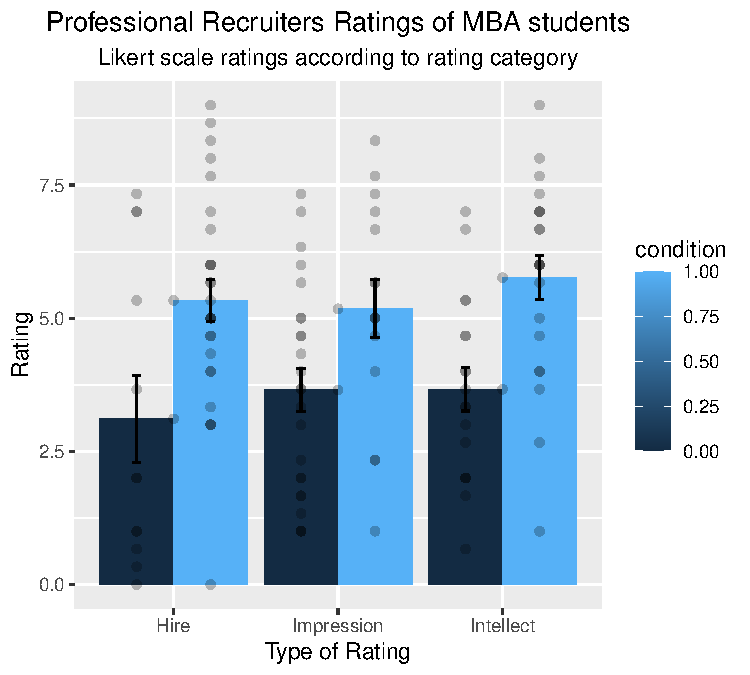
\includegraphics{Work_files/figure-latex/unnamed-chunk-2-1.pdf}
\caption{\label{fig:unnamed-chunk-2}Average ratings of MBA candidates according to specific categories}
\end{figure}

The results of this analysis indicates that main effect of pitch condition presentation exists for ratings of intellect, impression and hiring likelihood. Professional recruiters believed candidates with audio pitch presentation conditions had significantly larger intellect (M = 5.63, SD = 1.61) than those with transcribed pitch presentation conditions (M = 3.65, SD = 1.91) t(37) = -3.53, p = 0.001, two.sided. Similarly, the results indicated that candidates with audio pitch presentation conditions left a more positive and less negative impression on the recruiters (M = 5.97, SD = 1.92) than candidates with transcribed pitch presentation conditions (M = 4.07, SD = 2.23), t(37) = -2.85, p = 0.007, two.sided. Finally, recruiters had a greater likelihood of hiring candidates with audio pitch presentation conditions (M = 4.71, SD = 2.26) than those with transcribed pitch presentations (M = 2.89, SD = 2.05), t(37) = -2.62, p = 0.013, two.sided.

\hypertarget{discussion}{%
\section{Discussion}\label{discussion}}

This analysis indicates the existence of evidence of vocal communication being effective mechanism of perception formation. A potential explanation of these findings may be in the effectiveness of voices to convey aspects speech such as intonation, pacing and cadence. Seeing as how these aspects of speech enables for an effective communication of one's thoughts, it should also enable the formation of stronger perceptions of others mental capacity. These stronger perceptions may provide further explanations as to why candidates who used audio as a means of presenting their pitches were perceived as having a larger intellect, leaving a better impression and having a better hiring likelihood by professional recruiters than candidates who transcribed their pitch presentations.

\hypertarget{power-analysis}{%
\section{Power Analysis}\label{power-analysis}}

The experimental design of Schroder \& Epley (2015) was a single measures between subjects design with 39 professional recruiters. In this experimental design, a single main effect of pitch presentation is observed. 21 Participants experienced the audio pitch conditions while 18 subjects experience the transcribed pitch conditions.
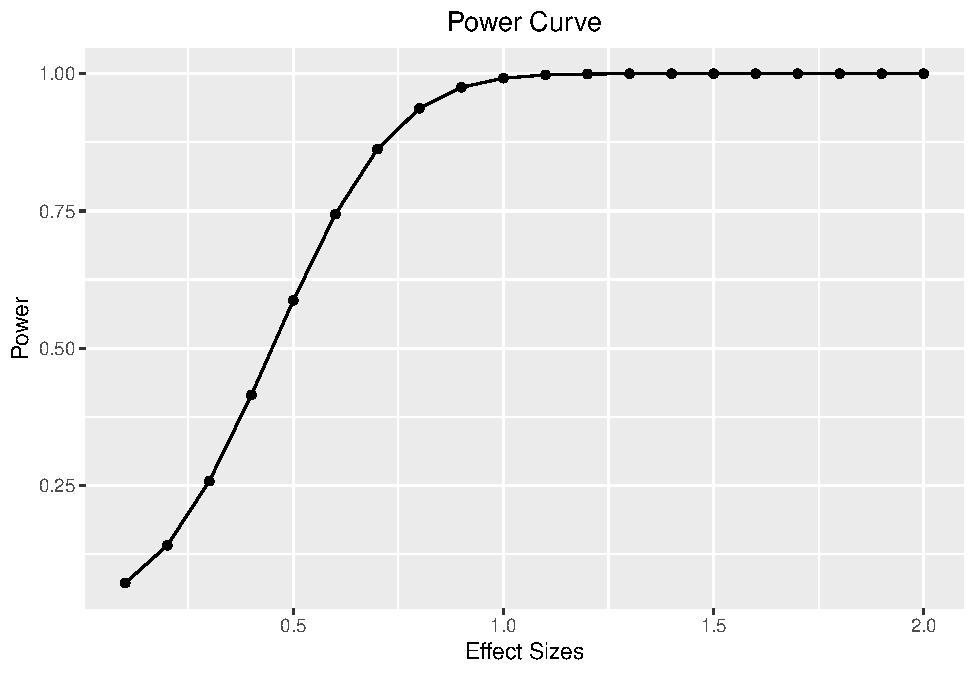
\includegraphics{Work_files/figure-latex/unnamed-chunk-3-1.pdf}
To detect the power of the experimental design, a power curve of a t-test for independent samples (n = 39) was created. This power curve shows the levels of power required to detect a range of effect sizes. The effect sizes range from 0.1 to 2.0 across intervals of 0.1. The power curve above finds that this design has a power of 0.99 to detect an effect of d = 1.0 and larger. The full power curve for this design is displayed in Figure 2

\newpage

\hypertarget{references}{%
\section{References}\label{references}}

\begingroup
\setlength{\parindent}{-0.5in}
\setlength{\leftskip}{0.5in}

\hypertarget{refs}{}
\leavevmode\hypertarget{ref-R-papaja}{}%
Aust, F., \& Barth, M. (2020). \emph{papaja: Prepare reproducible APA journal articles with R Markdown}. Retrieved from \url{https://github.com/crsh/papaja}

\leavevmode\hypertarget{ref-R-tinylabels}{}%
Barth, M. (2021). \emph{tinylabels: Lightweight variable labels}. Retrieved from \url{https://github.com/mariusbarth/tinylabels}

\leavevmode\hypertarget{ref-R-pwr}{}%
Champely, S. (2020). \emph{Pwr: Basic functions for power analysis}. Retrieved from \url{https://CRAN.R-project.org/package=pwr}

\leavevmode\hypertarget{ref-Hall_2007}{}%
Hall, J. A., \& Schmid Mast, M. (2007). Sources of accuracy in the empathic accuracy paradigm. \emph{Emotion}, \emph{7}(2), 438--446. \url{https://doi.org/10.1177/0956797615572906}

\leavevmode\hypertarget{ref-kruger2005egocentrism}{}%
Kruger, J., Epley, N., Parker, J., \& Ng, Z.-W. (2005). Egocentrism over e-mail: Can we communicate as well as we think? \emph{Journal of Personality and Social Psychology}, \emph{89}(6), 925.

\leavevmode\hypertarget{ref-R-base}{}%
R Core Team. (2020). \emph{R: A language and environment for statistical computing}. Vienna, Austria: R Foundation for Statistical Computing. Retrieved from \url{https://www.R-project.org/}

\leavevmode\hypertarget{ref-schr_SoundofInt}{}%
Schroeder, J., \& Epley, N. (2015). Sources of accuracy in the empathic accuracy paradigm. \emph{Emotion}. \url{https://doi.org/10.1177/0956797615572906}

\leavevmode\hypertarget{ref-R-plyr}{}%
Wickham, H. (2011). The split-apply-combine strategy for data analysis. \emph{Journal of Statistical Software}, \emph{40}(1), 1--29. Retrieved from \url{http://www.jstatsoft.org/v40/i01/}

\leavevmode\hypertarget{ref-R-ggplot2}{}%
Wickham, H. (2016). \emph{Ggplot2: Elegant graphics for data analysis}. Springer-Verlag New York. Retrieved from \url{https://ggplot2.tidyverse.org}

\leavevmode\hypertarget{ref-R-dplyr}{}%
Wickham, H., François, R., Henry, L., \& Müller, K. (2021a). \emph{Dplyr: A grammar of data manipulation}. Retrieved from \url{https://CRAN.R-project.org/package=dplyr}

\leavevmode\hypertarget{ref-R-readr}{}%
Wickham, H., Hester, J., \& Bryan, J. (2021b). \emph{Readr: Read rectangular text data}. Retrieved from \url{https://CRAN.R-project.org/package=readr}

\endgroup


\end{document}
